\chapter{Cumulative Impact of other EIs and RFIs}
\newthought{A growing list of Engineer's Instructions and Requests for Information} followed-up, the signing of the Memorandum of Agreement. The growth of the EIs is shown graphically in Figure~\ref{EIplots}. As at the end of May 2011, there were 300 EIs issued and 1054 RFIs.
Not only the Engineer failed to complete his design by the 15th of December 2009, as agreed with the Contractor and recorded in the Contractor's approved 6.2 Programme of Works, but the Engineer continued with changes well into a year after the planned Completion Date.


\def\monthnames{{"D","J","F","M","A","M","J","J","A","S","O","N","D"}}
\pgfplotsset{width=16cm}

\begin{fullwidth}
\begin{figure*}[htbp]
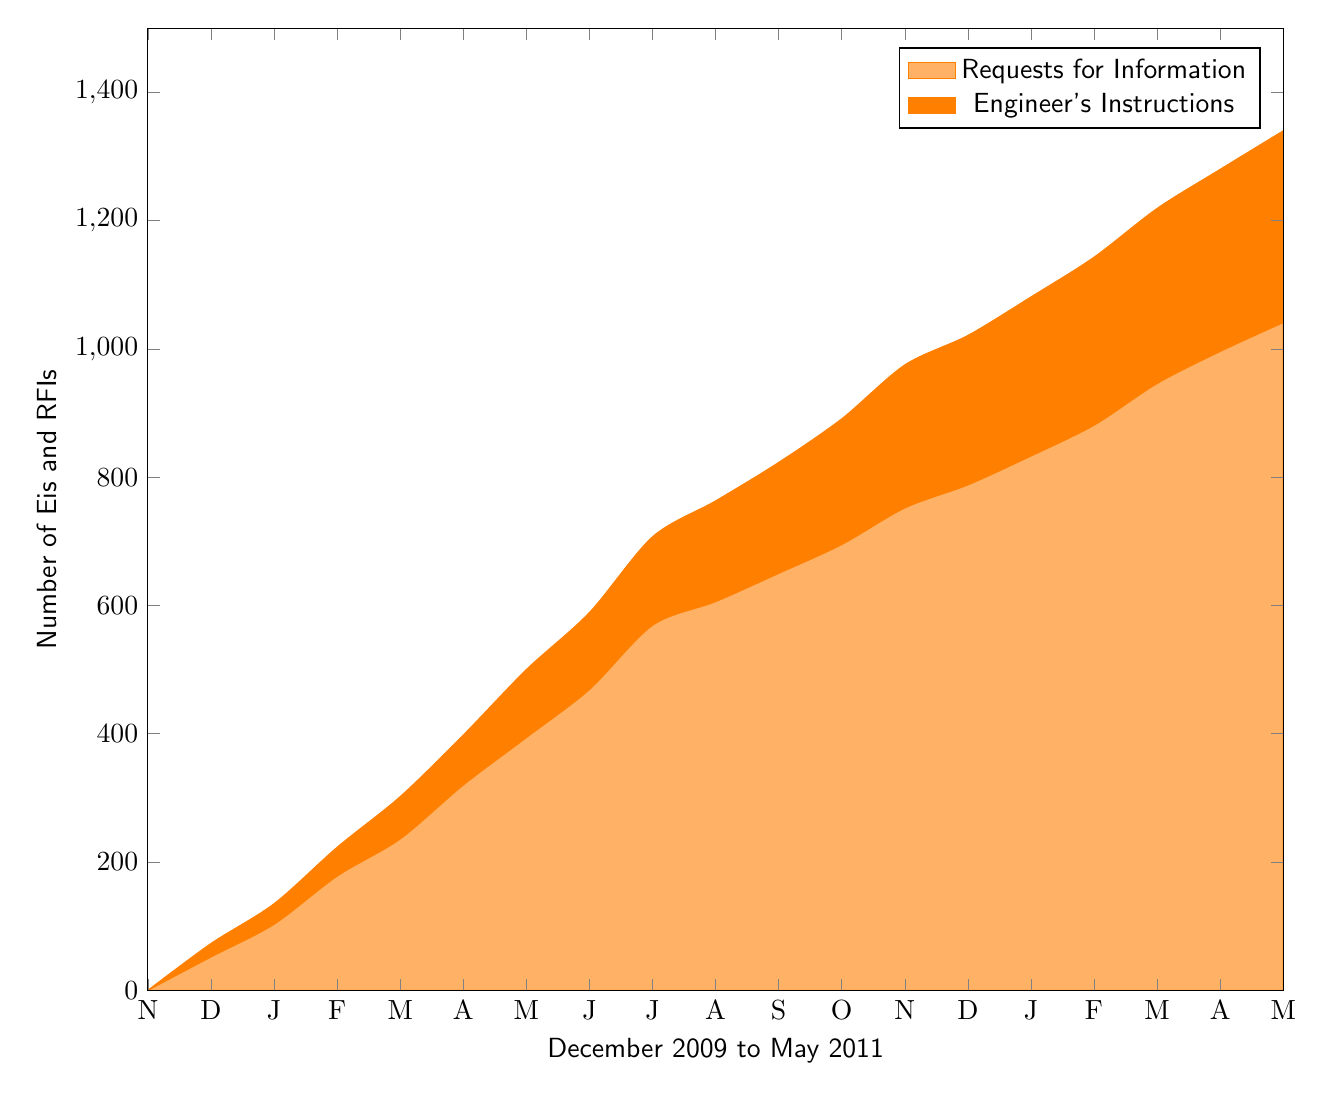
\begin{tikzpicture}
    \begin{axis}[
        smooth,
        stack plots=y,
        area style,
        enlarge x limits=false,
        ymin=0,ymax=1500,
        xlabel=\textsf{December  2009 to May 2011},
        ylabel=\textsf{Number of Eis and RFIs},
        xtick=data,
        %no need to repeat months more than a year
        xticklabel={\pgfmathparse{\monthnames[Mod(\tick-1,12)]}\pgfmathresult}]
\addplot[color=orange,fill=orange!60] coordinates
		{(0,0) (1,52) (2,103) (3,178) (4,236) (5,320) (6,394)%
                (7,469) (8,569) (9,606) (10,650) (11,695) (12,752)%
                (13,788) (14,833)  (15,881) (16,946) (17,996) (18,1041)
               } 
		\closedcycle;
	\addplot[color=orange,fill=orange] coordinates
		{(0,0) (1,21) (2,32) (3,45) (4,66) (5,78) (6,106)%
                (7,120) (8,138) (9,157) (10,173) (11, 196) (12,223)%
               (13,233) (14,248) (15,262) (16,273) (17,284) (18,299)
               }
		\closedcycle;
    \addlegendentry{\textsf{Requests for Information}}
    \addlegendentry{\textsf{Engineer's Instructions}}
    
   
 
    \end{axis}
\end{tikzpicture}
\caption{Plots showing the growth of Engineer's Instructions and their relationship to Requests for Information, the relationship can be observed clearly. See for example the \textit{bumps} at around April-May 2010.}
\label{EIplots}
\end{figure*}
\end{fullwidth}

No Project, where the Design is incomplete can be completed. It is obvious neither the Owner that could instruct the Engineer to add resources to his Team, nor the Engineer considered the Completion Date to be of \textit{essence}.

The Contractor on its part, accelerated works in sections that were critical for the Owners Direct Contractor to have access, providing this access at the end of June 2010.